% ------------- PREAMBLE ------------- %
% Currently using IEEEtran 1.8
\documentclass[10pt,conference,a4paper]{IEEEtran}
\usepackage{amsmath}
\usepackage{ucs}
\usepackage[utf8x]{inputenc}
\usepackage{times}
\usepackage{graphicx}
\setcounter{MaxMatrixCols}{30}
\usepackage{amsfonts}
\usepackage{amssymb}
\usepackage{url}
\usepackage{epstopdf}
% Style
\newcommand{\CLASSINPUTinnersidemargin}{18mm}
\newcommand{\CLASSINPUToutersidemargin}{12mm}
\newcommand{\CLASSINPUTtoptextmargin}{20mm}
\newcommand{\CLASSINPUTbottomtextmargin}{25mm}
\DeclareGraphicsExtensions{.png,.eps,.ps,.eps,.jpg}
% Hack para corregir las cabeceras de tablas de IEEEtran. Con esto figuras y tablas tienen el mismo formato.
\makeatletter \def\@IEEEtablestring{} \makeatother

% ------------- DOCUMENT ------------- %
\title{CARACTERIZACIÓN DE MEDIOS DE TRANSMISIÓN}
\author{
    \IEEEauthorblockN{Pablo Arrieta Nata, Daniel Iñigo Baños.}
    \IEEEauthorblockA{uo194468@uniovi.es, uo194823@uniovi.es.}
    \IEEEauthorblockA{Grado en Tecnologias y Servicios de Telecomunicación. Universidad de Oviedo.}
    \IEEEauthorblockA{Sistemas de Telecomunicación. Curso 2013-14.}
}
\begin{document}
\maketitle

\begin{abstract}
    Los medios de transmisión guiados y no guiados, como son el cable coaxial y el canal WiFi, presentan ventajas unos frente a otros en diferentes aspectos. Por esto, dependiendo del tipo de transmisión que se quiera realizar se emplea uno u otro. A continuación se estudian independientemente y se realiza una breve comparación a partir de su análisis en frecuencia.
\end{abstract}

% ------------------------------------------- %
% ------------- PRIMER MONTAJE  ------------- %
% ------------------------------------------- %
\section{Primer Montaje}
Empleando un analizador de redes se mide la respuesta en frecuencia de un cable coaxial mediante el parámetro $s_{2,1}$ en el ancho de banda de 1[MHz] a 2[GHz]. Se transmite una potencia de 0[dBm]. El $s_{2,1}$ representa la función de transferencia del cable en módulo-fase.
A partir de los datos experimentales se mide la atenuación que introduce el cable como $-H(f)$ y se compara con los del fabricante (tabla \ref{tab:atenuacion_coaxial}) y con el modelo teórico según la ecuación \ref{eq:atenuacion_coaxial}.
Se observa en la figura \ref{fig:atenuacion_comparada_coaxial} que la atenuación experimental se encuentra entre la que predice el modelo teórico y la que proporciona el fabricante. Esto se debe a que el modelo desprecia muchos factores que influyen en la atenuación y el fabricante trata de dar una cota superior de este añadiendo un margen.
La constnate de fase $\beta$ tiene como pendiente el tiempo de propagación. Está modelada por la ecuación \ref{eq:constante_fase_coaxial} . En la figura \ref{fig:constante_fase}. Normalizando este para que sean comparables.

La respuesta al impulso que calculamos es compleja y no causal. Hay que hace el módulo y eliminar la parte negativa del eje de tiempo. 

La velocidad de propagación por el cable se puede calcular como $$v_p = \frac{1}{t_d} = \frac{1}{4.55 [ns/m]} = 219.780 \cdot 10^6 [m/s]$$
Según el fabricante la velocidad de propagación es del $66 \%$ de la velocidad de la luz $$v_p = 0.66 \cdot 3 \cdot 10^8 [m/s] =  198 \cdot 10^6 [m/s]$$ Se tiene un error en la velocidad de propagación del $9.88 \%$ respecto al valor del fabricante.

\subsection{Ecuaciones}

\begin{eqnarray}
    \label{eq:atenuacion_coaxial}
    \alpha = \sqrt{\frac{\rho \omega \epsilon}{2}} \frac{\frac{1}{d_i} + \frac{1}{d_e}}{\ln{\frac{d_e}{d_i}}}
\end{eqnarray}

\begin{eqnarray}
    \label{eq:constante_fase_coaxial}
    \beta = \omega \sqrt{\mu \varepsilon}
\end{eqnarray}

\subsection{Figuras y Tablas}

\begin{table}[htb]
    \renewcommand{\arraystretch}{1.2}
    \centering
    % Number of cells must be declared when opening the table and so the separator.
    \begin{tabular}{|c|c|}
	\hline
	Frecuencia[MHz] & Atenuación [dB/100m] \\
	\hline
	1 & 1.3124 \\
	10 & 4.5934 \\
	50 & 10.8273 \\	
	100 & 16.0769 \\
	200 & 23.9513 \\
	400 & 37.7315 \\
	700 & 55.777 \\
	900 & 65.62 \\
	1000 & 70.5415 \\
	\hline
    \end{tabular}
    \caption{Atenuación en función de la frecuencia que proporciona el fabricante.}
    \label{tab:atenuacion_coaxial}
\end{table}

\begin{figure}[htb]
    \centering
    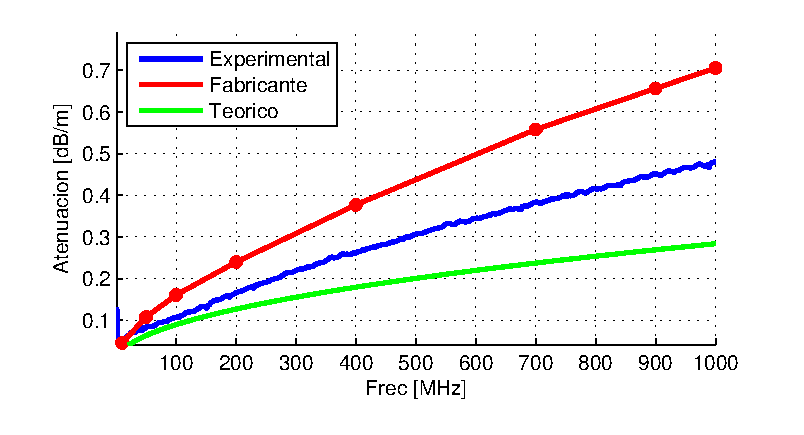
\includegraphics[width=\columnwidth]{figuras/atenuacion_comparada.eps}
    \caption{Atenuación por unidad de longitud en función de la frecuencia en un cable coaxial Belden}
    \label{fig:atenuacion_comparada_coaxial}
\end{figure}
\begin{figure}[htb]
    \centering
    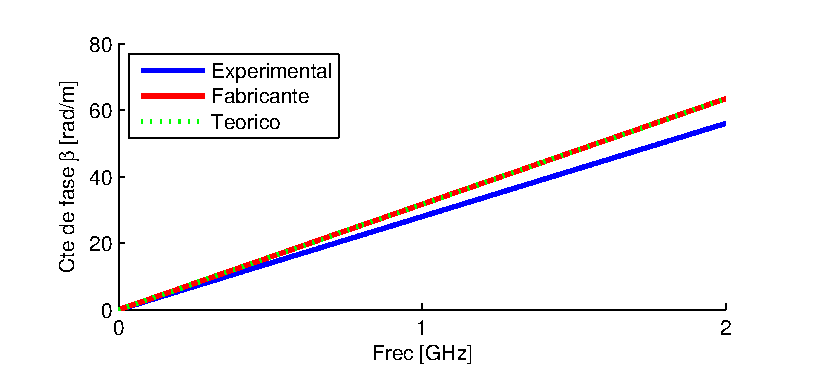
\includegraphics[width=\columnwidth]{figuras/constante_fase.eps}
    \caption{Atenuación por unidad de longitud en función de la frecuencia en un cable coaxial Belden}
    \label{fig:constante_fase}
\end{figure}
\begin{figure}[htb]
    \centering
    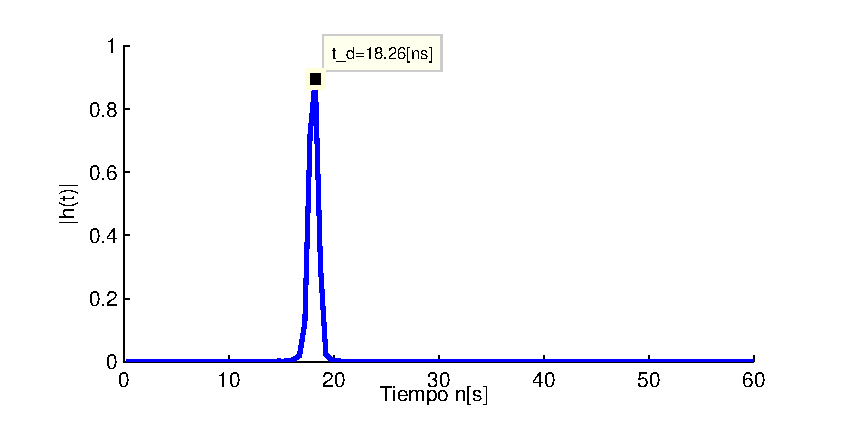
\includegraphics[width=\columnwidth]{figuras/respuesta_impulso.eps}
    \caption{Módulo de la respuesta al impulso del cable Belden de 4[m]}
    \label{fig:respuesta_impulso_coaxial}
\end{figure}
\begin{figure}[htb]
    \centering
    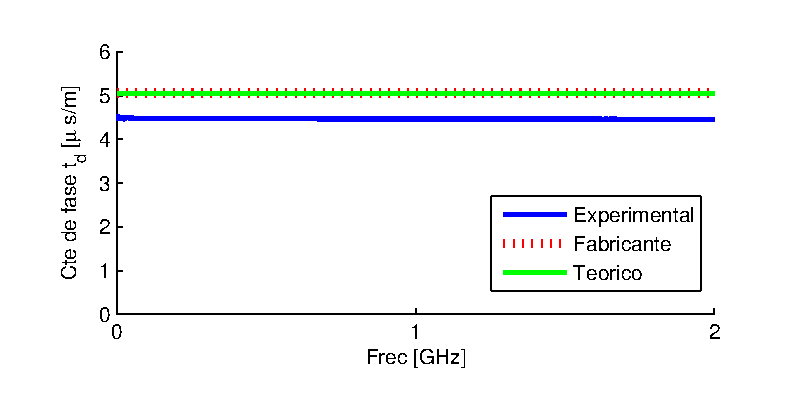
\includegraphics[width=\columnwidth]{figuras/retardo.eps}
    \caption{Atenuación por unidad de longitud en función de la frecuencia en un cable coaxial Belden}
    \label{fig:retardo_coaxial}
\end{figure}

% -------------------------------------------- %
% ------------- SEGUNDO MONTAJE  ------------- %
% -------------------------------------------- %
\section{Segundo Montaje}

\subsection{Figuras y Tablas}


\subsection{Ecuaciones}

\subsection{Numeración de páginas}

\subsection{Referencias}

Las referencias serán numeradas en orden de aparición [1]. El formato de
referencias será el estándar del IEEE. Se muestra algún ejemplo en el apartado correspondiente.

\subsection{Uno o más autores}

En caso de tener uno, dos o más de tres autores, adapte la zona
correspondiente a autores y afiliación de manera oportuna. Intente no variar
de manera notable el aspecto y tamaño de la zona.

\section{Conclusiones}

El seguimiento de las normas indicadas permitirá que su trabajo resulte
visualmente atractivo y que de lugar a impresiones de calidad. Esta misma
plantilla se puede encontrar en los formatos OpenDocument (ISO/IEC 26300:2006)
y Microsoft Word\textsuperscript{\textregistered} en la dirección web oficial del Simposium.

%Bibliografía

\begin{thebibliography}{9}                                                                                                %
    \bibitem {ref libro}C. Jones and K. Jones, \emph{How to publish a paper in 30
seconds,} 233rd ed., It is a Joke, Republic of Chiquitistan, 2009.

    \bibitem {ref articulo}K. Jones and L.Grijander, \textquotedblleft How to use
the copy and paste tool\textquotedblright\ Trans. on Phys. Rev., vol. 234, no.
7, pp. 635-646, Dec. 1935.
\end{thebibliography}


\end{document}
